%% REPLACE SXXXXXX with your student number
\def\studentNumber{S2026994}


%% START of YOUR ANSWERS
%% Add answers to the questions below, by replacing the text inside the brackets {} for \youranswer{ "Text to be replaced with your answer." }. 
%
% Do not delete the commands for adding figures and tables. Instead fill in the missing values with your experiment results, and replace the images with your own respective figures.
%
% You can generally delete the placeholder text, such as for example the text "Question Figure 2 - Replace the images ..." 
%
% There are 18 TEXT QUESTIONS (a few of the short first ones have their answers added to both the Introduction and the Abstract). Replace the text inside the brackets of the command \youranswer with your answer to the question.
%
% There are also 3 "questions" to replace some placeholder FIGURES with your own, and 3 "questions" asking you to fill in the missing entries in the TABLES provided. 
%
% NOTE! that questions are ordered by the order of appearance of their answers in the text, and not by the order you should tackle them. Specifically, you cannot answer Questions 2, 3, and 4 before concluding all of the relevant experiments and analysis. Similarly, you should fill in the TABLES and FIGURES before discussing the results presented there. 
%
% NOTE! If for some reason you do not manage to produce results for some FIGURES and TABLES, then you can get partial marks by discussing your expectations of the results in the relevant TEXT QUESTIONS (for example Question 8 makes use of Table 1 and Figure 2).
%
% Please refer to the coursework specification for more details.


%% - - - - - - - - - - - - TEXT QUESTIONS - - - - - - - - - - - - 



%% Question 1:
\newcommand{\questionOne} {
\youranswer{the train and validation accuracies initially increase as a function of epoch number. The same behaviour can be seen in figure 1b were train and validation errors are decreasing with one another. This observation is indicative of a model that is generalising well, as described in \citep[Ch.\ 5.2]{Goodfellow-et-al-2016}. At approximately 10 epochs one can see a sharp turn in the validation error. From this point on the errors diverge. This is typical of overparamaterised networks and is indicative of over-fitting \citep[Ch.\ 5.2]{Goodfellow-et-al-2016}. From this point on the train validation error gap increases with epoch number. Even when a network is generalising well, one still expects to see a small gap between the train and validation error. The fact that the validation error is increasing does however indicate that the model is overfitting. }
}

%% Question 2:
\newcommand{\questionTwo} {
\youranswer{the network with a hidden layer width of 32 units is the only network were overfitting is not apparent. This is indicated by the fact that both the train and validation errors are decreasing as a function of epoch number \citep[Ch. \ 5.2]{Goodfellow-et-al-2016}, despite a gap still being present. This is also apparent in the accuracy curves, were both the train and validation accuracies initially increase sharply before flattening off to a small positive gradient. Both the 64 and 128 width networks show this trend in their training curves. Their validation curves however show signs of overfitting due to their increasing value and divergence from the train error curve. One can see similarities between the overfit model in figure 1 and these models, namely that the validation errors deflect from a minima early on in the training and increase with subsequent epochs. The 128 width network shows this phenomena to a much greater degree, with a train validation error gap that is far more prominent than the 64 width network, as shown in table 1.}
}

%% Question 3:
\newcommand{\questionThree} {
\youranswer{
From the data observed in figure 2 and table 1, it does seem that network width has an effect on the degree to which the model overfits to the training data. Namely, that the wider networks overfit to a greater degree. This is in agreement with the general literature of the subject (as discussed in \citep{Bejani2021}). Wider, over-paramaterised neural networks have a greater capacity to explicitly remember the training data, even up to the point of remembering single, randomly mislabelled datapoints \citep{Zhang2016}. Hence they can over-fit by simply memorising all datapoints. 

 From observations made in this section, it is however not possible to determine if it's the width alone that causes this phenomena, or the fact that increasing the width introduces more free parameters that in turn causes the effect. It has generally been found that it's the number of model parameters (or more specifically model capacity) that increases the networks propensity for over-fitting \citep[Ch. \ 5.2, P. \ 112 - 113]{Goodfellow-et-al-2016}. 
 
 Interestingly, it is found that in the infite width limit neural networks have vastly different learning dynamics than in the finite limit \citep{Lee2019}. These models can approximate to guassian process and can in fact lead to better generalisation than models in the large width over-fitting regime. This has been verified empirically for very wide models. For our case, it is most likely that our models in the region of parameter space were they are over fitting, but not wide enough to operate in the regime described above.
 
 The final observation to note is that the validation error increases by approximately 2 to 3 times its optimal generalization value (located at approximately 10 ephocs), whereas the the validation accuracy barely decreases from its largest value. Here, the overfitting is manifesting as a probabilistic error (as discussed in \citep{Guo2017}). The model is generally still predicting the correct label, however due to the use of the cross entropy error, the models confidence in this prediction factors greatly into the error term, not just its value. The over-fit model is assigning larger probabilities to incorrect labels and lower probabilities to the correct labels than the well generalised model is. This is why the validation error of the 64 and 128 width models are far larger that of the 32 width model but the accuracies are not significantly smaller. 
 
 }
}

%% Question 4:
\newcommand{\questionFour} {
\youranswer{the validation error curves in figure 3b still show an increasing divergence from the train error curves for all 3 models. This is evidence that the models are still operating within the overfitting regieme for the 3 depths investigated. It's interesting to note that the gradient of the depth 2 model's validation error is much larger than that of the depth 1 model, but the difference between the depth 2 and depth 3 models is very small. This is also indicated by the similar train validation error gaps in table 2.
}
}

%% Question 5:
\newcommand{\questionFive} {
\youranswer{The findings above, that increasing the network depth increases the severity of over-fitting is consistent with the subject literature \citep[Ch. \ 5.2]{Goodfellow-et-al-2016}. The effect of increasing network depth does however not seem to increase the severity of over fitting as much as increasing width.

One explanation for this may simply stem from the fact that the depth 2 model may be at its maximum extent of over-paramaterisation. That is, the model has sufficient capacity to perfectly remember the training dataset (such as the models used in \citep{Zhang2016}). Adding more parameters to such a model increases it's capacity, but since the data is already memorised it's not going to substantially change the predictions of the trained model. For example, a quadritc model fitting 2 points, and a cubic model fitting 2 points could end up being the same, as the cubic model may train to set it's cubic exponent to 0. 

There is empirical evidence that very deep networks of the a similar complexity to a more traditional shallower models do tend to act better as universal approximators \cite{He2015}, so one may expect the deeper networks to over-fit the data to a greater degree. The fact that the depth 2 network is already very deep in the over fitting regieme means that this effect will not most likely increase as much in severity for subsequent depths.

It would ultimately be interesting to see what effect the depth and width have when the number of network paramaters are kept the same. It may be the case that a for a very narrow network bottlenecking \citep{Matejka2014}sets in and the network can again generalise better.
}
}





%% Question 6:
\newcommand{\questionSix} {
\youranswer{Table 3 shows the result of the experiments ran using different regularisation techniques and hyperparameter values.In this discussion, I will denote the Dropout, L1 penaly, L2 Penalty hyperparametes as $\lambda_d$, $\lambda_{L1}$, and $\lambda_{L2}$ respectively. 

Dropout layers seem to help mitigate the effect of over-fitting. One notes that the validation accuracy increases with dropout hyperparameter value. For $\lambda_{d} > 0.85$, the model beats the baseline for accuracy, and yields the joint best accuracy when $\lambda_d = 0.97$. Despite a validation train error gap still being present, it's substantially smaller that the baseline model, indicating that the model is generalising better. It is interesting to note that the gap increases as the model accuracy does. This relates to the explination in section 2.1, the model is obtaining the highest probability for the correct label but is more uncertain about it. For EMNIST classification purposes, accuracy is the most important metric, so the dropout models past $\lambda_d = 0.85$ are considered to be better than the baseline.

The L1 regularization seems to universally be worse than the baseline model, both in terms of accuracy and validation error. For values of $\lambda_{L1} < 10^{-3}$ the accuracy is still reasonable, but the train and validation errors are both larger than the baseline values. For greater $\lambda_{L1}$ values the validation accuracy drops to just above 2\%. Noting that the dataset has 47 distinct classes, this is close to the accuracy that a random guess would yield. It's clear here that the model has failed to train at all. The most likely explanation is that L1 term in the gradient is causing the model to take steps in loss space that are too large, causing it overshoot minima when performing gradient descent. This is bacause the L1 gradient term is always constant, so the gradient descent step size is bounded from below by $|\lambda_d|$ for each parameter. It is however interesting to note that for all hyperparameter values, the train validation error gap has closed. For the 2 larger $\lambda_{L1}$ values this is expected, as the model has failed to train. For the more accurate models this does indicate that the overfitting has been quelled, but unfortunately at the expense of model accuracy. It may be beneficial to investigate even smaller $\lambda_{L1}$ values, as the increased train error values indicate that the L1 term is not allowing the model to descend deep enough into the loss space minima.

The introduction of an L2 regularizer into the model seems to cause better generalisation than the baseline model. This is indicated by a reduction in the train validation error gap and a slight increase in the model accuracy. For increasing $\lambda_{L2}$ values, the gap does reduce, but at the expense of accuracy. This is again most likely due to regularizer not allowing the model to descend deep enough into the train loss space minima (as happened for the L1 model).

Finally, label smoothing seems to yield the joint best accuracy of all the models, but at the expense of both train and validation error. Recalling that the model outputs a probability mass function due to the final softmax term, the use of label smoothing can interpreted as decreasing the train label confidence. This in turn causes the model to factor this uncertainty into it's training, which as described earlier, manifests as an increased model error. It is clear however that this uncertainty has served to increase accuracy and generalization.

From the data gathered, models that beat the baseline accuracy are; the L2 model with ($\lambda_{L2} = 1e-3$ \& $\lambda_{L2} = 5e-4$), the label smoothing model with ($\alpha = 0.1$) and the dropout models for $\lambda_d = 0.97$ \& $\lambda_d = 0.85$.

From this analysis, I have chosen to test the dropout model ($\lambda_d = 0.97$) on the test dataset. I consider this to be better than the Label Smoothing model purely due to the smaller validation error term. The dropout model is more confident in its prediction than the Label Smoothing model is whilst obtaining the same accuracy. A test accuracy and test error of 84.8\% and 0.437 respectively was obtained. This is close the the validation values, and indicates that this model has indeed generalised well. 


}
}

%% Question 7:
\newcommand{\questionSeven} {
\youranswer{For 8 subsequent model assesments the hyperparameter combinations I would use can be found in \ref{tab:q7}. For the below investigations, I would keep the learning rate the same. This is to allow one to directly compare the investigations with the baseline and the previously assessed models.

\begin{table}[t]
    \centering
    \begin{tabular}{c|c|c}
    \toprule
        Model& Model& Hyperparameter \\ number & combination & values \\
        
                 
    \midrule
    \midrule
        \multirow{2}*{1}
                 & Dropout &  $\lambda_{d} = 0.97$    \\
                 & Label Smoothing  & $\alpha = 0.1$   \\
    \midrule
        \multirow{2}*{2}
                 & Dropout &  $\lambda_{d} = 0.97$    \\
                 & L2  & $\lambda_{L2} = 5e-4$   \\   
    \midrule
        \multirow{2}*{3}
                 & Label Smoothing &  $\alpha = 0.1$    \\
                 & L2  & $\lambda_{L2} = 5e-4$   \\ 
                 
    \midrule
        \multirow{3}*{4}
                 & Label Smoothing &  $\alpha = 0.1$    \\
                 & L2  & $\lambda_{L2} = 5e-4$   \\           
                 & Dropout &  $\lambda_{d} = 0.97$    \\
             
    \midrule
        \multirow{1}*{5}          
                 & Dropout &  $\lambda_{d} = 0.985$    \\
                 
        \multirow{1}*{6}          
                 & Dropout &  $\lambda_{d} = 0.91$    \\
                 
    \midrule
        \multirow{1}*{7}          
                 & Label Smoothing &  $\alpha = 0.05$    \\
                 
        \multirow{1}*{8}          
                 & Label Smoothing &  $\alpha = 0.15$    \\
   
   
 
    \bottomrule
    \end{tabular}
    \caption{A table showing the hyperparameter and model combinations I would investigate for 8 subsequent runs.}
    \label{tab:q7}
\end{table}


\begin{itemize}
\item \textbf{Model 1:} I would propose this combination as these were the 2 best performing models. It would be interesting to see if combining the 2 models yields better accuracy, or if the 2 techniques oppose one another and cause worse generalization.

\item \textbf{Model 2:} This is a combination of the best Dropout and best L2 model. I propose this investigation as it may be the case that some regularization techniques work better together than others.

\item \textbf{Model 3:} The motivation for this investigation is the same as for the previous model. Its simply investigating another combination of high performing models.

\item \textbf{Model 4:} This proposes testing the 3 best techniques together. If it is the case that the proposals above lead to better generalization, it may be the case that all 3 further increase the network performance.

\item \textbf{Models 5\& 6:} This proposed investigation serves to find the optimal value of $\lambda_d$. The models seem to get better for larger $\lambda_d$, although the baseline model is the same as $\lambda_d = 1$, so this cannot be the optimal value. This model is noticeably better ($\approx 2\%$), so I propose $\lambda_d = 0.985$ to scope the gap between this and the baseline model. I also propose a model with $\lambda_d = 0.91$ as this is in-between our existing datapoints. 0.97 is very close to 1, so it may well be the case that the optimal value of $lambda_d$ lies below 0.97.

\item \textbf{Models 7 \& 8:} I propose this investigation for the same reason. Label Smoothing seemed to be an effective technique to improve generalization and finding the optimal values of $\alpha$ would be beneficial. The reason I have proposed these specific values of $\alpha$ is to probe the space around the already evaluated model. As there is only one existing data point there isn't really a trend to follow.

\end{itemize}

General considerations for models 5,6,7 \& 8: When performing such investigations, one needs to be careful they aren't fitting hyperparamaters to the validation set. For this reason I would propose shuffling the training and validation sets between investigations, or possibly using K-Fold cross validation to attempt to mitigate this.

For further investigations I would propose testing other combinations to see if the optimal mixture and hyperparameter values can be found. It may be the case that suboptimal regularization techniques generalize better when employed with others, so testing these would be insightful. It would also be interesting to further investigate the optimal values for the hyperparameters when the the technique is employed on its own such as for models 5 - 8.

Finally, It may be interesting to see that happens if the baseline model is trained well beyond generalizaiton. It was recently noticed that overparamaterized models can suddenly generalize (and often very well) when trained far past the point of over fitting \citep{Power2022}. It could well be the case that this model exibits the same behaviour, and if so, it would be good to assess how well it generalizes. This is obviously a very inefficient way of training a model, but may be an interesting academic endeavour.
}
}



%% Question 8:
\newcommand{\questionEight} {
\youranswer{Initially the impact of network width and depth was investigated to see how these variables effected generalization. It was found that increasing the width past a certain point for a 1 layer network left it prone to overfitting and the model generalized poorly. It was discussed that this is indicated by a growing validation train error gap and a drop in validation accuracy. Subsequently, model depth was investigated and similar conclusions were drawn. Namely that deeper networks generalized worse up to a point, however increasing the depth past 2 layers did not seem to massively increase the overfitting. It was discussed that both these phenomena were most likely due to an increase in the number of network parameters, increasing its capacity and leaving it prone to overfitting.  These findings were consistent with the subject literature and is a well known phenomena in machine learning \citep[Ch.\ 5.2]{Goodfellow-et-al-2016} \citep{Bejani2021} \citep{Zhang2016}.

Next, a range of regularization techniques were investigated and compared against a baseline model. It was found that employing Dropout layers with a hyperparameter of $\lambda_d = 0.97$ and a Label Smoothing with $\alpha = 0.1$ both gave the best validation accuracies of 85.4\% (baseline was 83.7\%). L2 regularization was also found to yield a better validation (85.1 \%) accuracy than baseline model. The best performing model was determined to be the Dropout model. It was chosen over the Label Smoothing as it had lower train and validation errors. This yielded a test accuracy of 84.4\%, indicating that the technique allowed the previously overparamtereised network to generalise well.

Finally, further investigations were proposed. It was decided that further efforts should go towards investigating if combinations of the regularizing techniques lead to better generalization, or if their effects oppose one another. It was also discussed that finding the optimal hyperparameter values for the sucessful techniques would be beneficial. There would however need to be techniques implemented (such as K-Fold cross validation) to ensure one wasn't fitting hyperamaters to a specific validation set. It was also discussed that training well past the point of overfitting may also yield spontaneous generalization \citep{Power2022}.
}
}

%% - - - - - - - - - - - - FIGURES - - - - - - - - - - - - 

%% Question Figure 2:
\newcommand{\questionFigureTwo} {
\youranswer{Question Figure 2 - Replace the images in Figure 2 with figures depicting the accuracy and error, training and validation curves for your experiments varying the number of hidden units.
%
\begin{figure}[t]
    \centering
    \begin{subfigure}{\linewidth}
        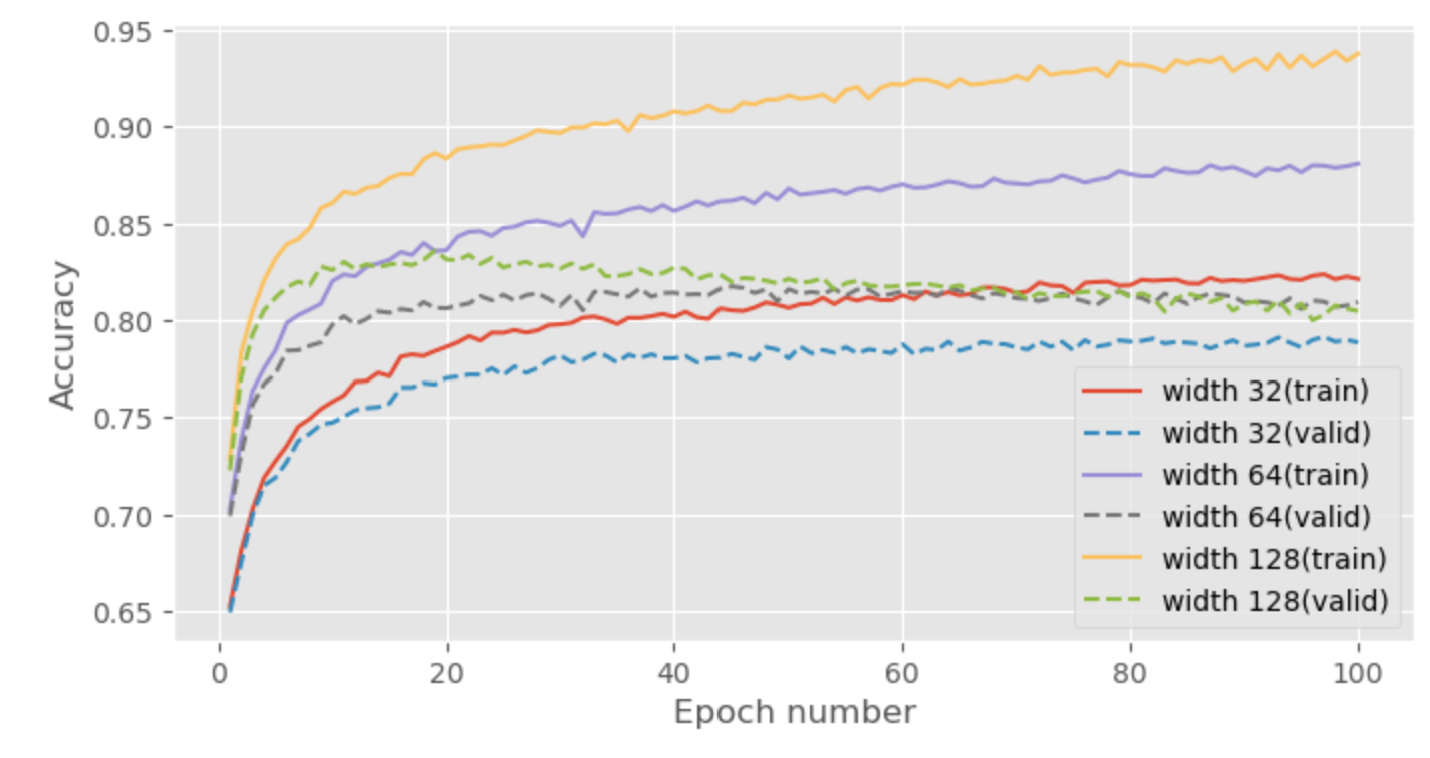
\includegraphics[width=\linewidth]{figures/acc_curve_width.png}
        \caption{accuracy by epoch}
        \label{fig:width_acccurves}
    \end{subfigure} 
    \begin{subfigure}{\linewidth}
        \centering
        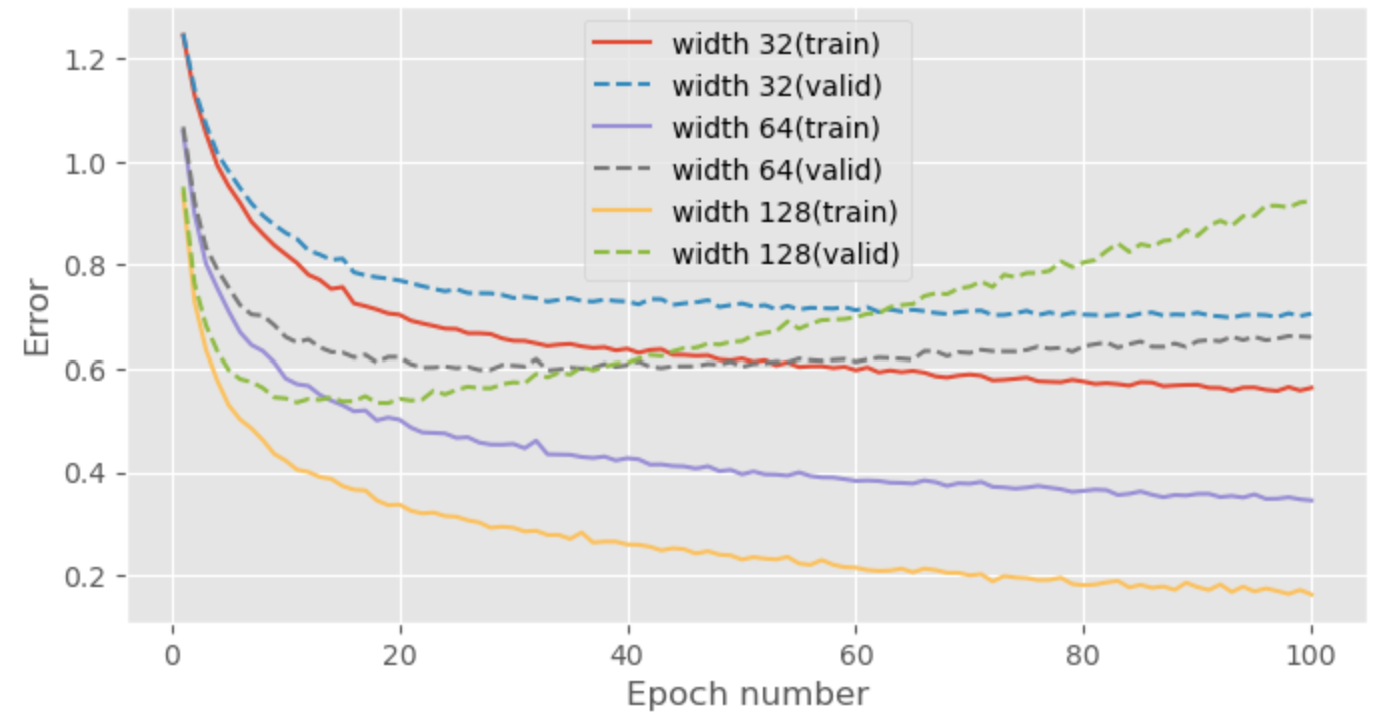
\includegraphics[width=\linewidth]{figures/error_curve_width.png}
        \caption{error by epoch}
        \label{fig:width_errorcurves}
    \end{subfigure} 
    \caption{Training and validation curves in terms of classification accuracy (a) and cross-entropy error (b) on the EMNIST dataset for different network widths.}
    \label{fig:width}
\end{figure} 
}
}

%% Question Figure 3:
\newcommand{\questionFigureThree} {
\youranswer{Question Figure 3 - Replace these images with figures depicting the accuracy and error, training and validation curves for your experiments varying the number of hidden layers.
%
\begin{figure}[t]
    \centering
    \begin{subfigure}{\linewidth}
        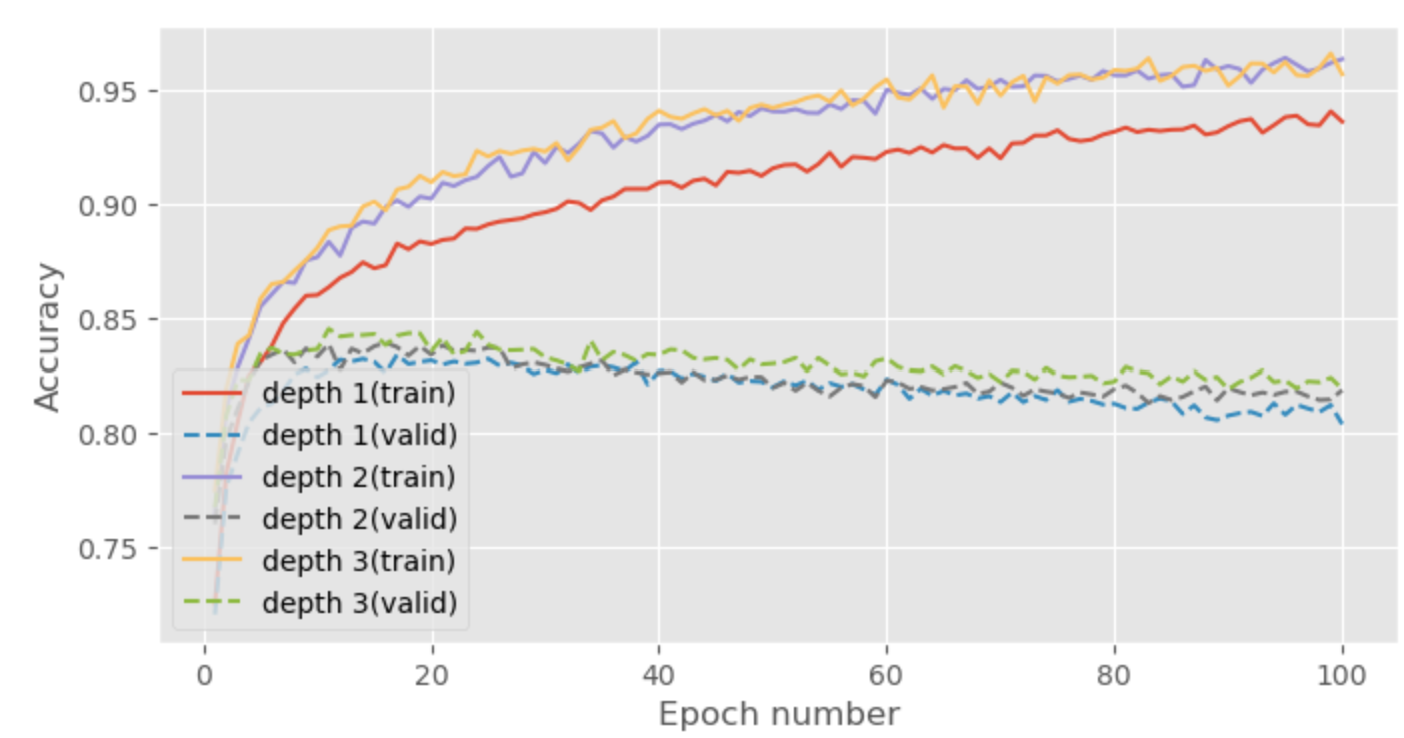
\includegraphics[width=\linewidth]{figures/acc_curve_depth.png}
        \caption{accuracy by epoch}
        \label{fig:depth_acccurves}
    \end{subfigure} 
    \begin{subfigure}{\linewidth}
        \centering
        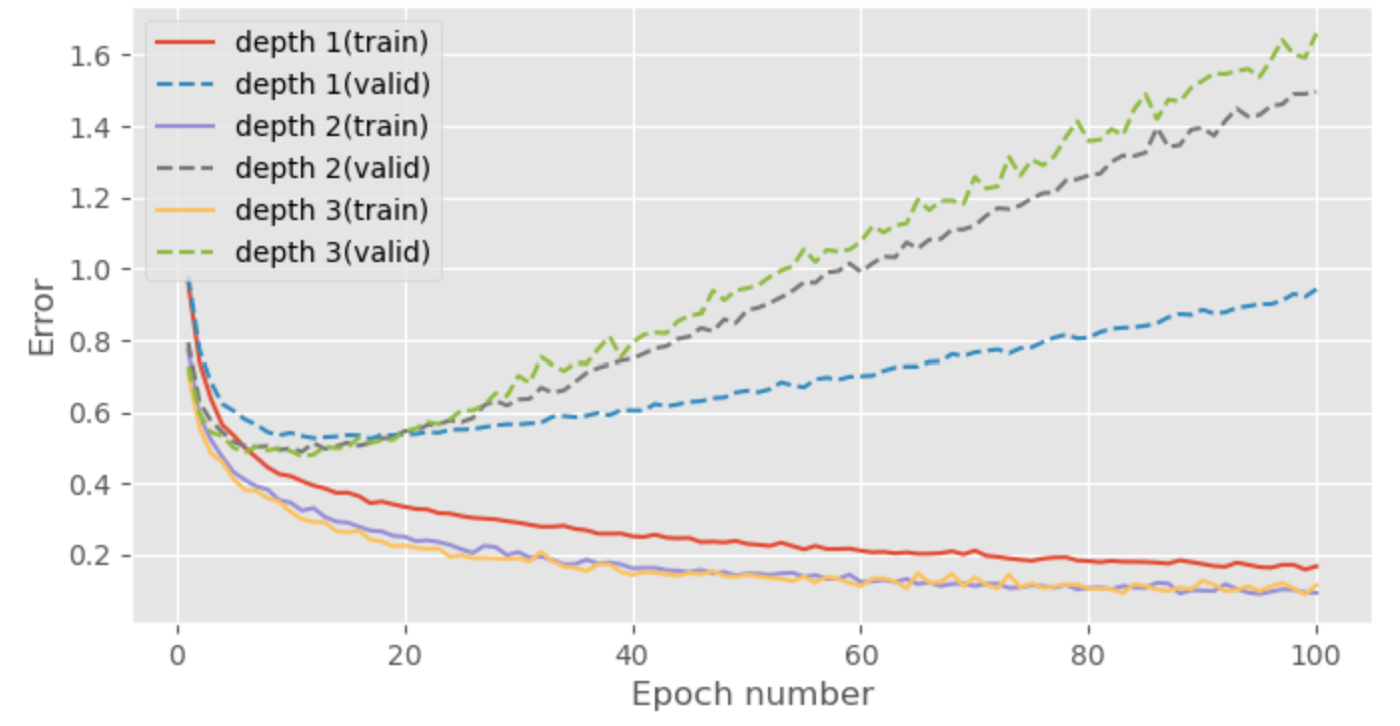
\includegraphics[width=\linewidth]{figures/error_curve_depth.png}
        \caption{error by epoch}
        \label{fig:depth_errorcurves}
    \end{subfigure} 
    \caption{Training and validation curves in terms of classification accuracy (a) and cross-entropy error (b) on the EMNIST dataset for different network depths.}
    \label{fig:depth}
\end{figure} 
}
}

%% Question Figure 4:
\newcommand{\questionFigureFour} {
\youranswer{Question Figure 4 - Replace these images with figures depicting the Validation Accuracy and Generalisation Gap (difference between validation and training error) for each of the experiment results varying the Dropout inclusion rate, and L1/L2 weight penalty depicted in Table 3 (including any results you have filled in).
%
\begin{figure*}[t]
    \centering
    \begin{subfigure}{.475\linewidth}
        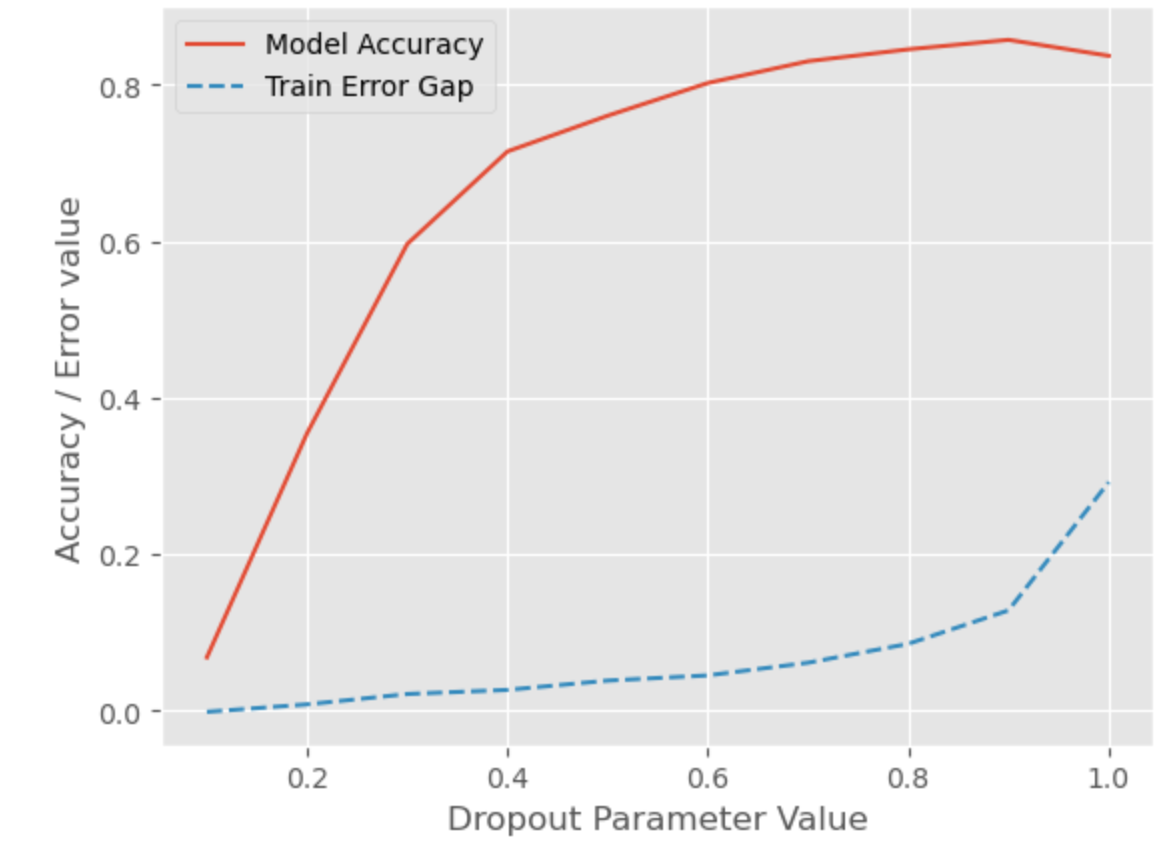
\includegraphics[width=\linewidth]{figures/dropout_plot.png}
        \caption{Accuracy and error by inclusion probability.}
        \label{fig:dropoutrates}
    \end{subfigure} 
    \begin{subfigure}{.475\linewidth}
        \centering
        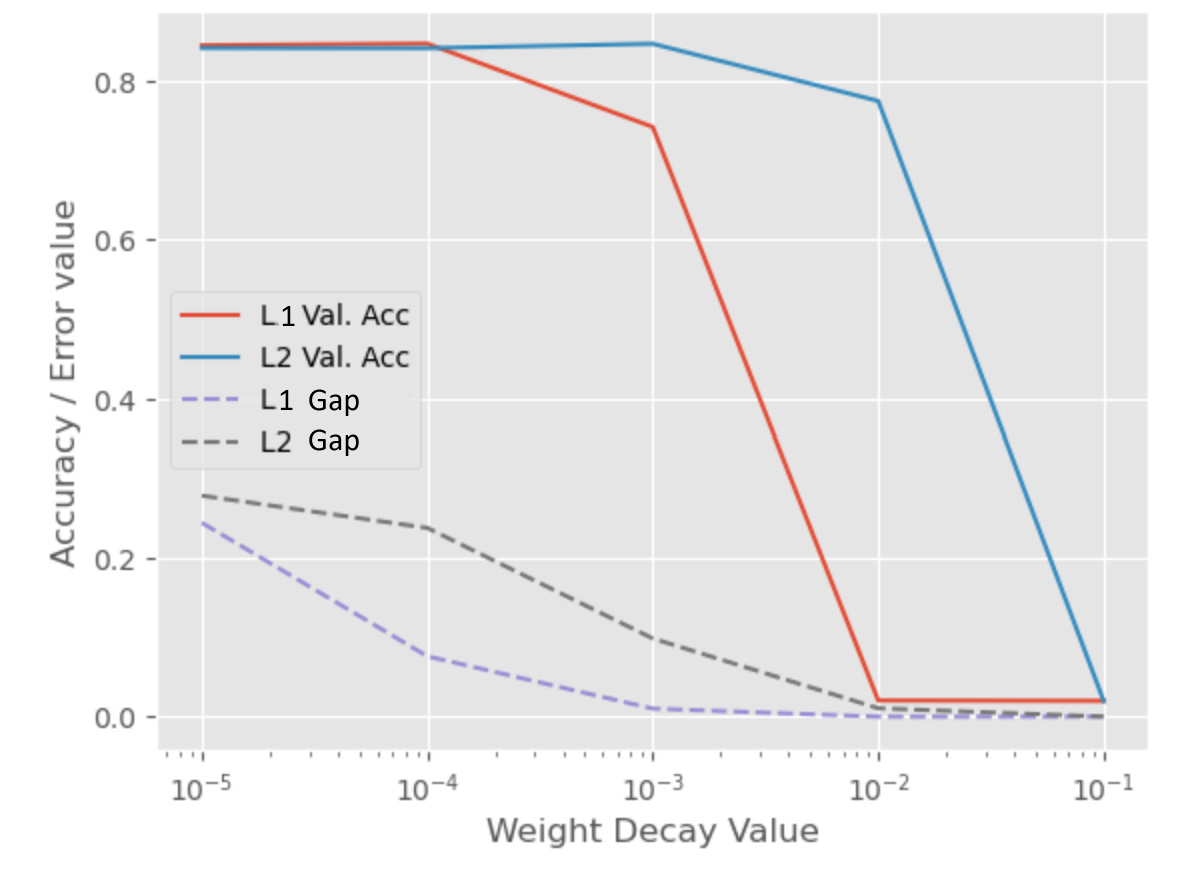
\includegraphics[width=\linewidth]{figures/wd_plot.png}
        \caption{Accuracy and error by weight penalty.}
        \label{fig:weightrates}
    \end{subfigure} 
    \caption{Accuracy and error by regularisation strength of each method (Dropout and L1/L2 Regularisation).}
    \label{fig:hp_search}
\end{figure*}
}
}

%% - - - - - - - - - - - - TABLES - - - - - - - - - - - - 

%% Question Table 1:
\newcommand{\questionTableOne} {
\youranswer{
Question Table 1 - Fill in Table 1 with the results from your experiments varying the number of hidden units.
%
\begin{table}[t]
    \centering
    \begin{tabular}{c|ccc}
    \toprule
        \# Hidden Units & Val. Acc. & Train Error & Val. Error\\
    \midrule
         32            &    78.8   &  0.525 &   0.705            \\
         64            &    80.5   &  0.336  &   0.678               \\
         128           &    80.8   &  0.161  &   0.936           \\ 
    \bottomrule
    \end{tabular}
    \caption{Validation accuracy (\%) and training/validation error (in terms of cross-entropy error) for varying network widths on the EMNIST dataset.}
    \label{tab:width_exp}
\end{table}
}
}

%% Question Table 2:
\newcommand{\questionTableTwo} {
\youranswer{
Question Table 2 - Fill in Table 2 with the results from your experiments varying the number of hidden layers.
%
\begin{table}[t]
    \centering
    \begin{tabular}{c|ccc}
    \toprule
        \# Hidden Layers & Val. Acc. & Train Error & Val. Error \\
    \midrule
         1               &      80.4      &   0.167 & 0.942                \\
         2               &      81.9      &   0.092 & 1.500                \\
         3               &      81.9      &   0.141 & 1.660                \\ 
    \bottomrule
    \end{tabular}
    \caption{Validation accuracy (\%) and training/validation error (in terms of cross-entropy error) for varying network depths on the EMNIST dataset.}
    \label{tab:depth_exps}
\end{table}
}
}

%% Question Table 3:
\newcommand{\questionTableThree} {
\youranswer{
Question Table 3 - Fill in Table 3 with the results from your experiments for the missing hyperparameter values for each of L1 regularisation, L2 regularisation, Dropout and label smoothing (use the values shown on the table).
%
\begin{table*}[t]
    \centering
    \begin{tabular}{c|c|ccc}
    \toprule
        Model    &  Hyperparameter value(s) & Validation accuracy & Train Error & Validation Error \\
    \midrule
    \midrule
        Baseline &  -                    &               0.837 &       0.241 &  0.533          \\
    \midrule
        \multirow{4}*{Dropout}
                 & 0.6                   &  80.7                &      0.549 & 0.593     \\
                 & 0.7 & 82.8 & 0.447 & 0.508  \\
                 & 0.85 & 85.1 &  0.329 &  0.434 \\
                 & 0.97 & 85.4 &  0.244 & 0.457  \\
    \midrule
        \multirow{4}*{L1 penalty}
                 & 5e-4 & 79.5 & 0.642 & 0.658 \\
                 & 1e-3 & 74.0 & 0.871 & 0.879 \\
                 & 5e-3 & 2.41 & 3.850 & 3.850 \\
                 & 5e-2 & 2.20 & 3.850 & 3.850 \\
    \midrule
        \multirow{4}*{L2 penalty}  
                 & 5e-4 & 85.1 & 0.306 & 0.460 \\
                 & 1e-3 & 85.1 & 0.357 & 0.451 \\
                 & 5e-3 & 81.3 & 0.586 & 0.607 \\
                 & 5e-2 & 39.2 & 2.258 & 2.256  \\
    \midrule
        Label smoothing & 0.1 & 85.4 & 1.020 & 1.151 \\
    \bottomrule
    \end{tabular}
    \caption{Results of all hyperparameter search experiments. \emph{italics} indicate the best results per series (Dropout, L1 Regularisation, L2 Regularisation, Label smoothing) and \textbf{bold} indicates the best overall.}
    \label{tab:hp_search}
\end{table*}
}
}



%% END of YOUR ANSWERS